%20 min preso!
\documentclass[xcolor=table]{beamer}
\usepackage{beamerthemesplit}
\usepackage{wrapfig}
\usetheme{SPbGU}
\usepackage{pdfpages}
\usepackage{amsmath}
\usepackage{cmap}
\usepackage[T2A]{fontenc}
\usepackage[utf8]{inputenc}
\usepackage[english]{babel}
\usepackage{indentfirst}
\usepackage{amsmath}
\usepackage{tikz}
\usepackage{multirow}
\usepackage[noend]{algpseudocode}
\usepackage{algorithm}
\usepackage{algorithmicx}
\usepackage{fancyvrb}
\usepackage{verbatim}
\usetikzlibrary{calc}
\usetikzlibrary{shapes,arrows}
\usetikzlibrary{arrows,automata}
\usetikzlibrary{positioning}

\usepackage{tabularx}
\newcolumntype{Y}{>{\raggedleft\arraybackslash}X}

\renewcommand{\thealgorithm}{}

\newtheorem{mytheorem}{Theorem}
\renewcommand{\thealgorithm}{}

\newcommand{\tikzmark}[1]{\tikz[overlay,remember picture] \node (#1) {};}
\def\Put(#1,#2)#3{\leavevmode\makebox(0,0){\put(#1,#2){#3}}}

\newcommand{\ltz}{$< 1$}


\tikzset{
    state/.style={
           rectangle,
           rounded corners,
           draw=black, very thick,
           minimum height=2em,
           inner sep=2pt,
           text centered,
           },
}

\beamertemplatenavigationsymbolsempty

\title[Formal Grammars + Neural Networks]{On Secondary Structure Analysis by Using
Formal Grammars and Artificial Neural
Networks}
%\subtitle[YaccConstructor]{Parsing techniques for graph analysis}
% То, что в квадратных скобках, отображается в левом нижнем углу.
\institute[]{
JetBrains Research, Programming Languages and Tools Lab  \\
Saint Petersburg University
}

% То, что в квадратных скобках, отображается в левом нижнем углу.
\author[Polina Lunina]{Semyon Grigorev, \textbf{Polina Lunina}}

\date{September 6, 2019}

\begin{document}
{
\begin{frame}[fragile]
  \begin{table}
  \centering
  \begin{tabularx}{\linewidth}{YcX}
    
\includegraphics[height=1.5cm]{pictures/jetbrainsResearch.pdf} \hfill
    & \begin{minipage}[t]{0.3\textwidth}\center \vspace{-1cm}  CIBB 2019
      \end{minipage}
    & \hfill 
\includegraphics[height=1.5cm]{pictures/SPbGU_Logo.png}
  \end{tabularx}
  \end{table}
  \titlepage
\end{frame}
}

\begin{frame} \frametitle{Genomic sequences analysis}
\begin{tabular}{cl}  
    \parbox{0.44\linewidth}{
        \begin{itemize}
            \item Problems
            \begin{itemize}
                \item Genomic sequences classification
                \item Subsequences detection
                \item Secondary structure prediction
            \end{itemize}
            \item Secondary structure handling
            \begin{itemize}
                \item Covariance models
                \item Hidden Markov Models
                \item Probabilistic grammars
            \end{itemize}
            \item Probability estimation for noisy data processing
        \end{itemize}
    }
    & \begin{tabular}{l}
            \vspace{-0.8cm}
            \hspace{-0.8cm}
            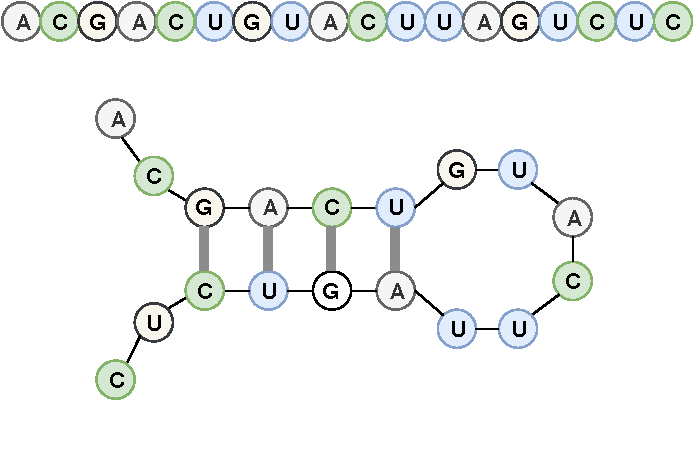
\includegraphics[width=6.5cm]{pictures/molekula.pdf}
         \end{tabular}  \\
\end{tabular}
\end{frame}

\begin{frame} \frametitle{Solution Structure}
\tiny %\hspace{-2cm}
  \begin{tikzpicture}[->,>=stealth']


  \node[state,
        align=left,
        text width = 3.5cm] (grm)
   {
    \textbf{Grammar}\\
  Fixed formal grammar (not necessarily context-free) describes features of secondary structure.

   };

  \node[state,
        below of=grm,
        node distance=1.2cm,
        align = left,
        text width = 3.5cm] (sqs)
   {
   \textbf{Sequences}\\
  Each sequence is treated as a text in $\{A, C, G, U\}$ alphabet.
   };


  \node[state,
        right of=grm,
        node distance=4cm,
        align = left,
        text width = 3.5cm](parser)
  {
  \textbf{Parser}\\
  Parser extracts features of the given sequence secondary structure.
  Implementation of parsing algorithm is based on matrix multiplications (Valiant, Okhotin) and utilizes GPGPU.
  };

  \node[state,
        right of=parser,
        node distance=4cm,
        align = left,
        text width = 3.5cm] (mtrx)
  {
    \textbf{Matrices}\\
    %\vspace{0.05cm}
    \[ \left( \begin{array}{cccc}
    0 & \textbf{1} & 0 & \textbf{1}\\
    0 & 0 & \textbf{1} & 0\\
    0 & 0 & 0 & \textbf{1}\\
    0 & 0 & 0 & 0
    \end{array} \right)\]
    \vspace{-0.1cm}

  Parsing result is a boolean matrix~$M$ which represents secondary structure features for sequence $\omega$: $ M[i,j] = 1 \iff \text{\ttfamily{s1}} \xrightarrow{*}{} \omega[i,j]$, and $0$ otherwise.
  };

  \node[state,
        below of=sqs,
        node distance=1cm,
        align = left,
        text width = 3.5cm](result)
  {
  \textbf{Result of classification}

  };


  \node[state,
        below of=parser,
        node distance=4.1cm,
        align = left,
        text width = 3.5cm](DNN)
  {
  \textbf{Neural Network}\\

  Dense neural network with more than 10 dense layers.
  Aggressive dropout and batch normalization for learning process stabilization.\\
  Typical building block:
  \\
  \vspace{-0.3cm}
  \begin{center}
  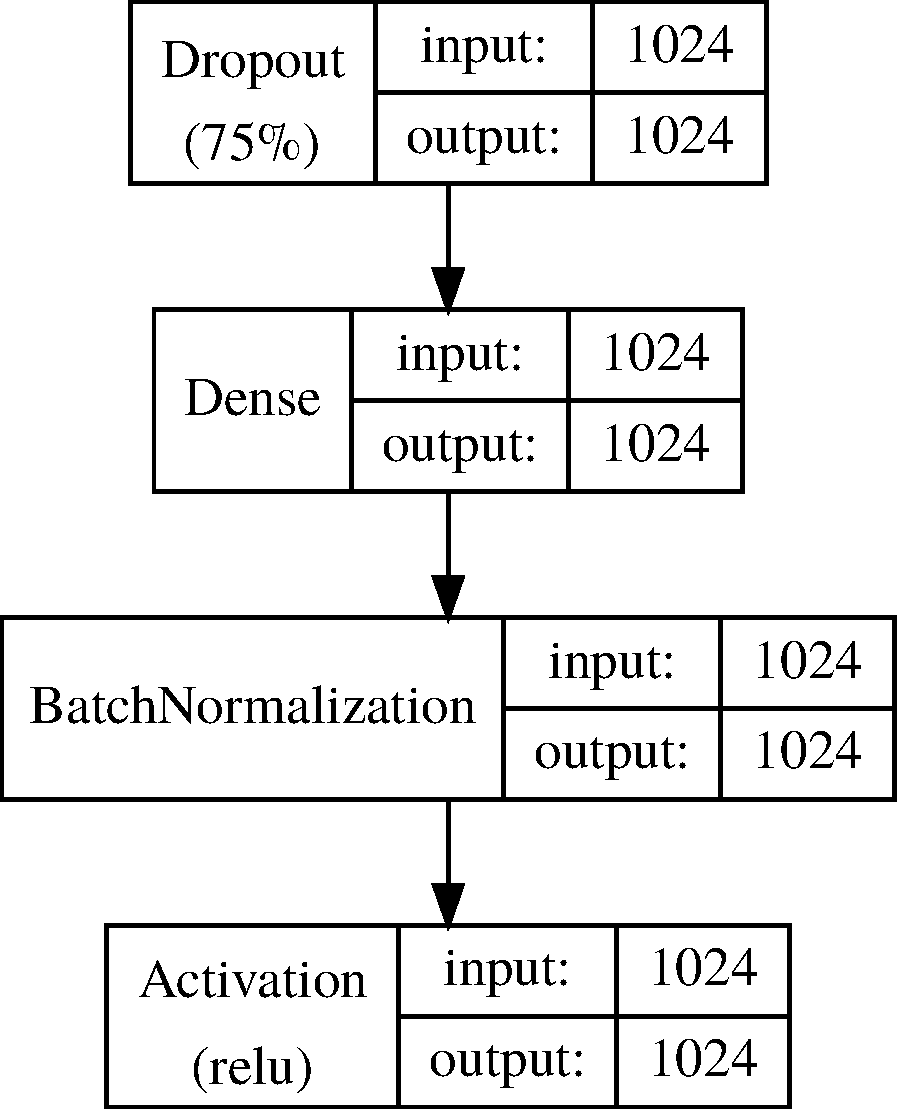
\includegraphics[width=2.5cm]{pictures/bb.pdf}
  \end{center}

  };


  \node[state,
        right of=DNN,
        node distance=4cm,
        align = left,
        text width = 3.5cm](vector)
  {
  \textbf{Vectors}\\
  \vspace{-0.1cm}

\[ \left( \begin{array}{cccc}
0 & 1 & 0 & 1\\
0 & 0 & 1 & 0\\
0 & 0 & 0 & 1\\
0 & 0 & 0 & 0
\end{array} \right) \]
\vspace{-0.35cm}
$$\Downarrow$$
\vspace{-0.35cm}
$$\texttt{[0,1,0,1,0,1,0,0,1,0]}$$
\vspace{-0.35cm}
$$\Downarrow$$
\vspace{-0.35cm}
$$\texttt{[84,128]}$$
%\vspace{-0.1cm}
  Line-by-line compressed matrix representation: sequence of 8 cells (bits) is compressed into a byte. Bottom left triangle of the matrix is always empty, so, it can be ignored.
  };


  \path (grm) edge  (parser)
   (sqs.east) edge [bend right=10] (parser.south)
   (parser) edge (mtrx)
   (mtrx) edge (vector)
   (vector) edge (DNN)
   (DNN.west) edge [bend left] (result.south)
   ;

  \end{tikzpicture}

  \tikzmark{zzz}{
  }
  %}
  \pause
  \onslide<2>{\tikz[overlay,remember picture]{\draw[draw=red,thick,double,fill opacity=0.2, rounded corners] ($ (zzz) + (-0.0,7.35)$) rectangle ($ (zzz) + (3.7,5.1)$);}}

  \onslide<3>{\tikz[overlay,remember picture]{\draw[draw=red,thick,double,fill opacity=0.2, rounded corners] ($ (zzz) + (4.0,7.7)$) rectangle ($ (zzz) + (7.7,5.85)$);}}

  \onslide<4>{\tikz[overlay,remember picture]{\draw[draw=red,thick,double,fill opacity=0.2, rounded corners] ($ (zzz) + (8.0,8.35)$) rectangle ($ (zzz) + (11.7,5.2)$);}}

  \onslide<5>{\tikz[overlay,remember picture]{\draw[draw=red,thick,double,fill opacity=0.2, rounded corners] ($ (zzz) + (8.0,4.95)$) rectangle ($ (zzz) + (11.7,0.4)$);}}

  \onslide<6>{\tikz[overlay,remember picture]{\draw[draw=red,thick,double,fill opacity=0.2, rounded corners] ($ (zzz) + (4.0,5.1)$) rectangle ($ (zzz) + (7.7,0.3)$);}}

  \onslide<7>{\tikz[overlay,remember picture]{\draw[draw=red,thick,double,fill opacity=0.2, rounded corners] ($ (zzz) + (-0.0,4.85)$) rectangle ($ (zzz) + (3.65,4.3)$);}}

\end{frame}


\begin{frame}{Example}
\centering
 \texttt{CCCC{\color{red}AUUGCCAAGG}ACCCCA{\color{red}CCUUGGCAAU}CCC}
\vspace{1cm}

\tikzmark{xx}{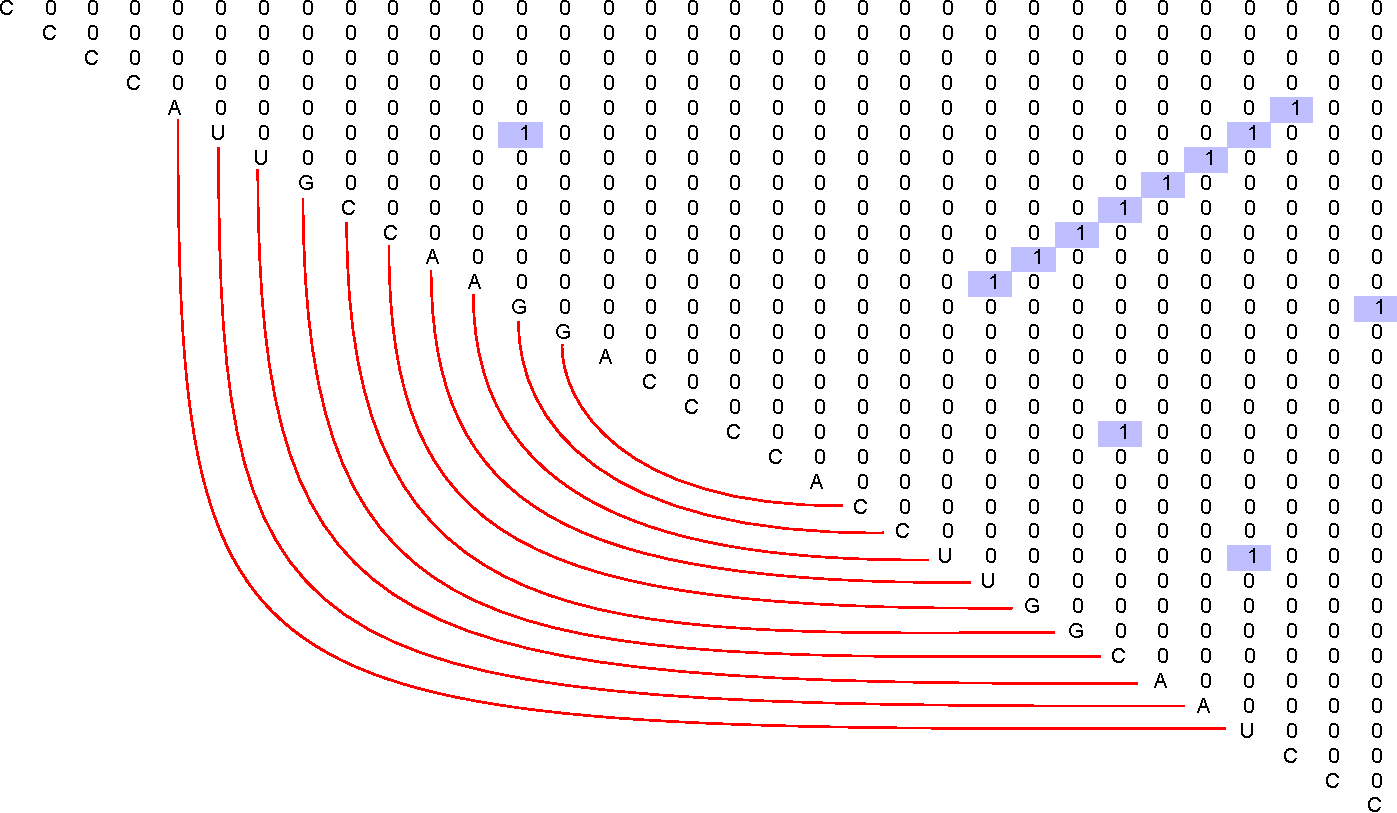
\includegraphics[width=.8\textwidth]{pictures/mtr.pdf}}
\onslide<2-3>{
\tikz[overlay,remember picture]{
\draw[draw=red,thick,fill opacity=0.2] ($(xx) + (1.1,4.97)$) rectangle ($(xx) + (9.05,3.235)$);
}
}

\onslide<3>{
\tikz[overlay,remember picture]{
\draw[draw=red,thick,fill opacity=0.2] ($(xx) + (5.8,4.97)$) rectangle ($(xx) + (8.75,0.4)$);
}
}
\end{frame}


\begin{frame}{Data locality preservation}
    \begin{itemize}
        \item Represent parsing result as an image
        \item Use convolutional layers for these images processing
        \item Compare image- and vector-based networks on the same data
    \end{itemize}
\end{frame}

\begin{frame}{Parsing results representation}
\tiny %\hspace{-2cm}
  \begin{tikzpicture}[->,>=stealth']

  \node[state,
        align = left,
        text width = 5.5cm] (mtrx)
  {
    \textbf{Matrices}\\
    %\vspace{0.05cm}
    \[ \left( \begin{array}{ccccc}
    0 & 1 & 0 & ... & 1\\
    0 & 0 & 1 & ... & 0\\
    0 & 0 & 0 & ... & 1\\
    ... & ... & ... & ... & ...\\
    0 & ... & ... & ... & 0
    \end{array} \right)\]
    \vspace{-0.1cm}

  Parsing result is a boolean matrix~$M$ which represents secondary structure features for sequence $\omega$: $ M[i,j] = 1 \iff \text{\ttfamily{s1}} \xrightarrow{*}{} \omega[i,j]$, and $0$ otherwise.
  };

  \node[state,
        right of=mtrx,
        node distance=6.5cm,
        align = left,
        text width = 5.5cm](vector)
  {
  \textbf{Vectors}\\
  \vspace{-0.1cm}


$$\texttt{[1,0,...,1,1,...,0,...,1,...]}$$
\vspace{-0.35cm}
$$\Downarrow$$
\vspace{-0.35cm}
$$\texttt{[84,128,...]}$$
%\vspace{-0.1cm}
  Line-by-line compressed matrix representation: sequence of 8 cells (bits) is compressed into a byte. Bottom left triangle of the matrix is always empty, so can be ignored. Requires the equal length of the input sequences and breaks the data locality.
  };

\node[state,
      line width=0.5mm,
      below = 1 of mtrx,
      node distance=3cm,
      align = left,
      text width = 5.5cm](image)
{
\textbf{Images}\\
\vspace{-0.2cm}
\begin{center}
\fbox{
\includegraphics[width=1.5cm]{pictures/bmp.png}}
\end{center}
The false bits of the matrix are represented as white pixels and the true bits as black ones. This approach makes it possible to process sequences of different lengths since the images can be transformed to a specified size. Data locality is preserved.

};


  \path 
   (mtrx) edge (vector)
   (mtrx.south) edge (image.north)
   ;

  \end{tikzpicture}
\end{frame}


\begin{frame}{Parsing elimination}
    \begin{itemize}
        \item Create a network which handles initial sequences
        \item Use two-staged learning
        \begin{itemize}
            \item Train network on images or vectors for a given problem
            \item Extend it by several input layers that take the initial nucleotide sequence as an input and convert it to the parsing result 
        \end{itemize}
    \end{itemize}
\end{frame}

\begin{frame}{Neural networks}
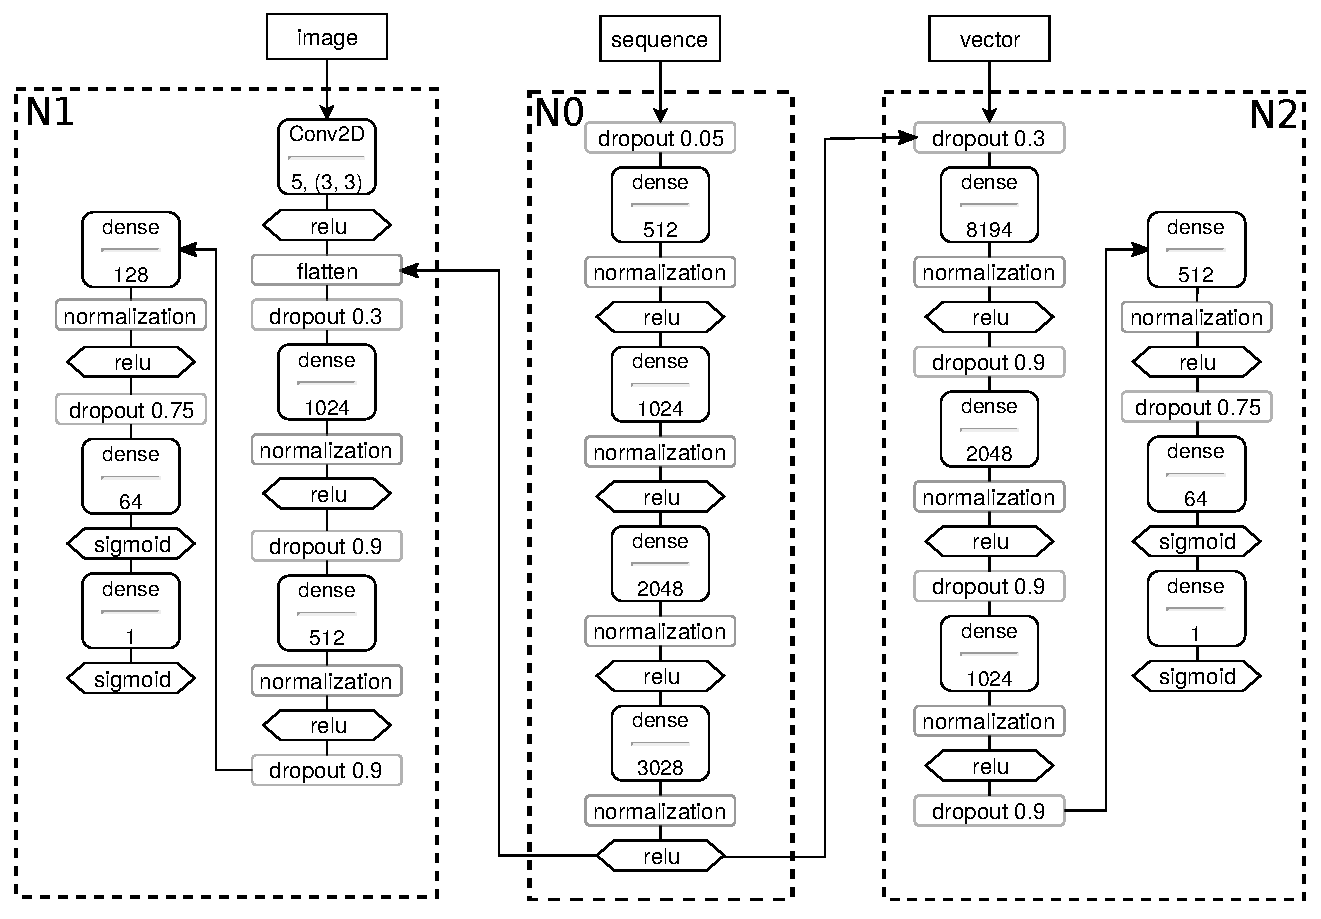
\includegraphics[width=11.5cm]{pictures/nn_arch.pdf}
\end{frame}


\begin{frame}{Evaluation}
\begin{itemize}
    \item tRNA sequences analysis tasks
    \begin{itemize}
        \item Classification into two classes: eukaryotes and prokaryotes
        \item Classification into four classes: archaea, bacteria, plants and fungi
    \end{itemize}
    \item Databases
    \begin{itemize}
        \item tRNADB-CE
        \item Genomic tRNA database
    \end{itemize}
\end{itemize}
\end{frame}

\begin{frame}{Results}
EP --- eukaryotes/prokaryotes task

ABFP --- archaea/bacteria/plants/fungi task

\begin{table}[h]
\centering
\caption{Base and extended models test results by accuracy metrics}
\begin{tabular}{|l||l|l||l|l|}
\hline
Classifier                                                               & \multicolumn{2}{l||}{EP}               & \multicolumn{2}{l|}{ABFP}           \\ \hline \hline
Approach                                                                 & Vector-based       & Image-based      & Vector-based      & Image-based     \\ \hline
\begin{tabular}[c]{@{}l@{}}Base model\\ accuracy\end{tabular}            & 94.1\%             & 96.2\%           & 86.7\%            & 93.3\%          \\ \hline
\begin{tabular}[c]{@{}l@{}}Extended model \\ accuracy\end{tabular}       & 97.5\%             & 97.8\%           & 96.2\%            & 95.7\%          \\ \hline
\begin{tabular}[c]{@{}l@{}}Total training \\ time\end{tabular}       & 30000s             & 4600s           & 31800s            & 3600s          \\ \hline
\begin{tabular}[c]{@{}l@{}}Samples for\\ train:valid:test\end{tabular} & \multicolumn{2}{l||}{\begin{tabular}[c]{@{}l@{}}20000:5000:10000\\ (57\%:14\%:29\%)\end{tabular}} & \multicolumn{2}{l|}{\begin{tabular}[c]{@{}l@{}}8000:1000:3000\\ (67\%:8\%:25\%)\end{tabular}} \\ \hline
\end{tabular}
\label{acc}
\end{table}

\end{frame}

\begin{frame}{Results}
EP --- eukaryotes/prokaryotes task

ABFP --- archaea/bacteria/plants/fungi task

\begin{table}[h]
\scriptsize
\centering
\begin{tabular}{|l||l|l|l|l|l|}
\hline
\multirow{2}{*}{Classifier} & \multirow{2}{*}{Class} & \multicolumn{2}{l|}{Vector-based approach} & \multicolumn{2}{l|}{Image-based approach} \\ \cline{3-6} 
                            &                        & precision         & recall        & precision        & recall        \\ \hline \hline
\multirow{2}{*}{EP}         & prokaryotic            & 95.8\%            & 99.4\%        & 96.2\%           & 99.4\%        \\ \cline{2-6} 
                            & eukaryotic             & 99.4\%            & 95.6\%        & 99.4\%           & 99.5\%        \\ \hline \hline
\multirow{4}{*}{ABFP}       & archaeal               & 91.1\%            & 99.2\%        & 91.6\%           & 98.5\%        \\ \cline{2-6} 
                            & bacterial              & 96.6\%            & 95.1\%        & 95.2\%           & 95.5\%        \\ \cline{2-6} 
                            & fungi                  & 98.5\%            & 94.9\%        & 97.5\%           & 94.3\%        \\ \cline{2-6} 
                            & plant                  & 99.4\%            & 95.7\%        & 99.2\%           & 94.7\%        \\ \hline
\end{tabular}
\end{table}
\end{frame}

\begin{frame}{Conclusion}
\begin{itemize}
    \item The modifications of our approach for biological sequences analysis were implemented
    \begin{itemize}
        \item Parsing result in a form of image can be handled by convolutional layers
        \item The parsing step can be removed from the trained model use which allows to run models on the original RNA sequences        
    \end{itemize}
    \item These modification improve the quality of the solution
    \item The improved version is applicable for real-world problems
\end{itemize}
\end{frame}

\begin{frame}{Future work}
\begin{itemize}
    \item Other RNA sequences analysis tasks
    \begin{itemize}
        \item 16s rRNA classification
        \item Chimeric sequences filtration
    \end{itemize}
    \item Secondary structure prediction by using generative networks
    \item The use of deep convolutional networks for secondary structure analysis
\end{itemize}

\end{frame}

\begin{frame}
\frametitle{Contact Information}
\begin{itemize}
  \item Semyon Grigorev:
    \begin{itemize}
      \item \href{mailto:s.v.grigoriev@spbu.ru}{s.v.grigoriev@spbu.ru}
      \item \href{mailto:Semen.Grigorev@jetbrains.com}{Semen.Grigorev@jetbrains.com}
    \end{itemize}
  \item Polina Lunina: \href{mailto:lunina\_polina@mail.ru}{lunina\_polina@mail.ru}
  \item Secondary structure analyzer project: \href{https://research.jetbrains.org/groups/plt\_lab/projects?project\_id=43}{https://research.jetbrains.org/groups/plt\_lab/projects?project\_id=43}
\end{itemize}
\vspace{0.3cm}
\center{\huge{Thanks!}}
\end{frame}
\end{document}
